\documentclass[abstract=on,9pt,twocolumn]{scrartcl}

\usepackage{ucs}
\usepackage[utf8x]{inputenc}
\usepackage[T1]{fontenc}
\usepackage[english]{babel}

%\usepackage{graphics}%	images other than eps

\usepackage[paper=a4paper,top=2cm,left=1.5cm,right=1.5cm,bottom=2cm,foot=1cm]{geometry}

\usepackage{relsize}%	relative font sizes

\usepackage[retainorgcmds]{IEEEtrantools}%	IEEEeqnarray
\setlength{\IEEEnormaljot}{4\IEEEnormaljot}

\usepackage{graphicx}
\usepackage{epstopdf}
\usepackage{indentfirst}
\usepackage{hyperref}
%\usepackage{cleveref}
\usepackage[noabbrev]{cleveref}
\usepackage{listings}
\usepackage{color}

%%%%%%%%%%%%%%%%
%  title page  %
%%%%%%%%%%%%%%%%
\titlehead{University of Minho \hfill Master's Degree in Informatics Engineering\\	Department of Informatics \hfill Parallel and Distributed Computing}

\title{Parallel Sorting}

\subtitle{Samplesort with Regular Sampling}

\author{Pedro Costa \hfill--- \texttt{\smaller pg19830@alunos.uminho.pt}}

\date{Braga, May 2012}

\subject{Parallel Computing Paradigms}


%%%%%%%%%%%
%  Hacks  %
%%%%%%%%%%%

%	Paragraph (title) with linebreak
\newcommand{\paragraphh}[1]{\paragraph{#1\hfill}\hfill

}

%	Add "Appendix" to the appendices titles, but not to the references
\usepackage{ifthen}
\newcommand*{\appendixmore}{%
  \renewcommand*{\othersectionlevelsformat}[1]{%
    \ifthenelse{\equal{##1}{section}}{\appendixname~}{}%
    \csname the##1\endcsname\autodot\enskip}
  \renewcommand*{\sectionmarkformat}{%
    \appendixname~\thesection\autodot\enskip}
}




\begin{document}
\maketitle

\section{Introduction}
%	1.	Contextualização
The sorting problem consists in finding a permutation $B$ for a sequence $A$, of $n$ elements, such that
$$\forall i,j \in \left \{ 1 , \ldots , n \right \} : i \leq j \Leftrightarrow b_{i} \leq b_{j}\enspace .$$

Many algorithms exist to solve this problem in a sequential fashion, from the purely academic bubblesort (with complexity $O(n^{2})$ in the average case) to the non-comparative radix sort (applicable only with integer keys, it has $O(kn)$ in the average case). Yet, in the multicore era, new approaches are required to take advantage of the available parallellism. 

%	2.	Objectivos
This document aims to study a parallel sorting algorithm and describe two implementations: one in distributed memory with MPI, and another in shared memory with OpenMP. The two implementations are also to be compared regarding scalability and complexity.

%	Estrutura
\Cref{sec:algorithm} describes the chosen algorithm for this assignment. \Cref{sec:omp,sec:mpi} describe how each of the components in the algorithm was implemented. Finally, \cref{sec:compare} shows a small profiling made to compare both versions.

\section{PSRS}
\label{sec:algorithm}
The chosen algorithm to study in this document is the Parallel Sorting with Regular Sampling (PSRS) by \cite{Li1993}, also known as Samplesort. In PSRS, the domain is divided into $p$ disjoint partitions which can be handled in parallel. The strategy consists in eight specific steps:
\begin{description}
	\item[Partition]{The original sequence of $n$ elements is divided into $p$ partitions. How elements are distributed influences the load balance.}
	\item[Local sort]{Each partition is sorted using a sequential algorithm.}
	\item[Sampling]{From each partition, $p$ samples are collected at regular intervals.}
	\item[Pivots]{All the collected $p^{2}$ samples are gathered and sorted, and $p-1$ pivots are collected at regular intervals.}
	\item[Slices]{Each partition is divided into $p$ slices according to the pivots.}
	\item[Trade]{Each $k^{\mathrm{th}}$ gets the $k^{\mathrm{th}}$ slice from all the partitions (including itself). The resulting partitions reflect the division according to the pivots.}
	\item[Local sort (again)]{Each partition is, again, sorted using a sequential algorithm.}
	\item[Gather]{All the partitions are concatenated in an ascendent order. The resulting sequence is a sorted permutation of the original one.}
\end{description}

\begin{figure*}[t]
	\begin{center}
		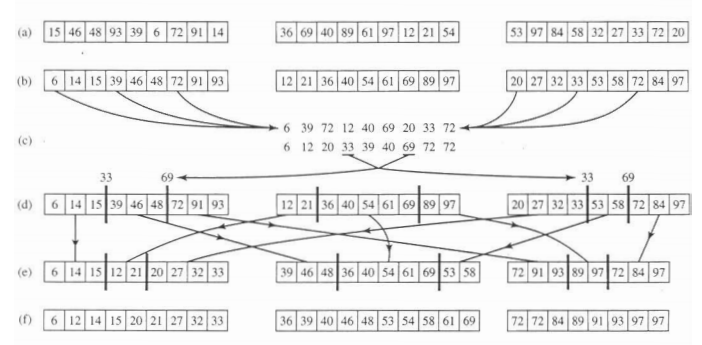
\includegraphics[width=\textwidth]{images/quinn.png}
	\end{center}
	\caption{``This example illustrates how three processors would sort 27 elements using the PSRS algorithm. (a) Original unsorted list of 27 elements is divided among three processes. (b) Each process sorts its share of the list using the sequential quicksort. (c) Each process selects regular samples from its sorted sublist. A single process gathers these samples, sorts them, and broadcasts pivot elements from the sorted list of samples to the other processes. (d) Processes use pivot elements computed in step (c) to divide their sorted sublists into three parts. (e) Processes use pivot elements computed in step (c) to divide their sorted sublists into three parts. (e) Processes perform an all-to-all communication to migrate the sorted sublist parts to the correct processes. (f) Each process merges its sorted sublists.'' -- from \cite{Quinn2004}, figure 14.5, page 347}
	\label{fig:quinn}
\end{figure*}

Variants of this algorithm change how the samples and/or pivots are collected and usually focus in reducing the amount of communication required.

According to \cite{Kale2010}, in comparison with the parallel Radix Sort, this algorithm presents excellent data movement (as each key is guaranteed to be moved once, at most), requires supplementary communication bandwidth only when collecting the samples (on very large systems, this value will increase by $\Omega(p^{2})$, has some ability to exploit a partially sorted initial distribution (inherited from quicksort) and is able of overlapping some of its communication with computation (this is harder with Regular Sampling).









\section{Distributed Memory}
\label{sec:mpi}
The version in distributed memory was implemented using OpenMPI. In this context, each process handles a different partition, and data transmission is done manually using communication directives (in contrast to having a global structure in memory). To create the analogy with the generic algorithm, this implementation works as follows:
\begin{description}
	\item[Partition]{The root process reads the file containing the keys to sort and stores them in an array. Taking the number of processes as the number of partitions, the array is divided in a round-robin fashion (assuring the closest to perfect load balance) and each partition is sent to the respective process.}
	\item[Local sort]{Each process uses the quicksort algorithm to locally sort its partition.}
	\item[Sampling]{Each process collects $p$ samples from its partition at defined intervals. 
	
	Contrary to what is defined in the original algorithm, in this implementation the interval is not constant. Instead, the intervals are calculated using the round-robin strategy. This assures that the intervals never differ by more than 1. Using a constant interval implies that either the first or the last sample (depends on which one is the starter sample) will not be evenly spaced like all the others.
	
	Each process ends this step by sending its samples to the root process.}
	\item[Pivots]{The root process gathers the samples from all the other processes, and sorts them using quicksort.
	
	Using the sorted keys, the root process repeats the sampling process to obtain $p-1$ pivots. The strategy used is exactly the same as in the Sampling step.
	
	At the end of this step, the root process broadcasts the array of pivots to the entire process pool.}
	\item[Slices]{According to the calculated pivots, each process divides its partition into $p$ slices. For each pivot $q_{k}$, the elements in slices $1,\ldots,k$ are less than or equal to the pivot. Obvious to say that the final slice will contain those elements greater than the last pivot.}
	\item[Trade]{After slicing the partition, every process will send each of its slices to the corresponding process. To avoid deadlocks, this is done in turns according to the process number. In each turn, the corresponding process sends its slices to all the other processes.\footnote{Such may be overcome using asynchronous communication. In MPI these correspond to the \texttt{ISend} and \texttt{IRecv} functions. Such was not implemented due to timeframe limitations in this project (the synchronous directives are easier to use).}.
	
	This step is performed in two similar phases: first only the slice sizes are sent, and only in the second phase are slices actually traded. This allows each process to allocate only the necessary memory for the resulting partition.}
	\item[Local sort (again)]{Each process uses the quicksort algorithm again to sort the resulting partition.
	
	After sorting, every process sends its partition to the root process.}
	\item[Gather]{The root process gathers the all the partitions and concatenates them into a new array in the same memory space as the original one (thus preventing one extra memory allocation).
	
	The algorithm ends with the root process outputting the sorted sequence.}
\end{description}



\subsection{Communication Complexity}
Implementing any algorithm in a distributed memory paradigm such as message passing with MPI allows any algorithm to be achieve a level of parallelism superior to the one with shared memory. Yet, while shared memory suffers from having less capacity for parallelism (limited by hardware components, whereas distributed memory is limited only by the number of available nodes), it also does not require communication external to the computational node.

Consequently, distributed algorithms are deeply influenced by communication. In addition to being CPU-bound or memory-bound, these algorithms may be communication-bound, which is directly influenced by the communication complexity. While analyzing the complexity it is assumed no other influence in the communication process aside from the parameters of the algorithm (number of keys to sort and number of partitions to use).

The PSRS algorithm requires communication in 5 occasions: when the root process sends the partitions to each process (Partition); when the samples are sent from every process to root (Sampling); when the root process broadcasts the pivots (Pivots); when every process trades slices with each other (Trade); and, lastly, when all the processes send their partitions to root (Gather).

In the Partition step, the root process sends the $n$ keys to the respective processes. For simplicity, we assume that the root process also sends the data to itself, therefore resulting in $O(n)\enspace .$

Sampling implies that all the $p$ processes sends its $p$ samples to the root process, which results in $O(p^{2})\enspace .$

At the end of the fourth step, the root process broadcasts the $p-1$ pivots. This results in $O(p(p-1))\enspace .$

The Trade step is the one which seems to have more communication, due to the all to all nature. Yet, each element of the original array will travel once at most. If, to simplify, is ignored that each process does not send its own slice to itself, the resulting complexity will be $O(n)\enspace .$

Lastly, the gather step is a mirror action of the partition step. Therefore its complexity is also $O(n)\enspace .$

Summing all the components, the resulting communication complexity is $$O(3n+p^{2}+(p-1)^{2})\enspace .$$












\section{Shared Memory}
\label{sec:omp}
OpenMP was used to implement the shared memory version of the algorithm. In contrast with the MPI version, this implementation compensates the lesser capacity for parallelism\footnote{In a cluster environment, MPI is able of using multiple computational nodes to its full capacity, whereas OpenMP is only able to use one computational node} with the absence of communication. Using global structures in the main memory, working threads are able to work without having to stop to exchange data.

In a similar way to the previous descriptions, this implementation works as follows:
\begin{description}
	\item[Partition]{The master thread reads the file containing the keys to sort and stores them in a global structure. The division into partitions is performed as in the MPI version.
	
	To note that the number of partitions is not necessarily the same as threads. Since hardware threads are usually limited to a small number, the number of partitions is allowed to be greater. The number of threads used in parallel regions is always the minimum between the number of hardware threads and the number of partitions. When the number of partitions exceeds the number of threads, static scheduling is used in a for loop to handle all the partitions.
	
	Each partition is represented by a size and an offset, both saved in global arrays.}
	\item[Local sort]{Each thread uses the quicksort on the partitions assigned to it.}
	\item[Sampling]{Each thread collects samples from the assigned partitions. The strategy is the same as in the MPI version. The collected samples are stored in a global array of $p^{2}$ elements.}
	\item[Pivots]{The master thread uses the quicksort algorithm to sort the array of samples and collects $p-1$ pivots, storing them in a global array. Again, the strategy is the same as used in the MPI version.}
	\item[Slices]{Each thread calculates where to slice its partition based on the array of pivots. Slices are represented in the same way as partitions (size and offset). Once more, the MPI strategy is reused.}
	\item[Trade]{Each thread accesses the global structure to retrieve the slices of its partitions. To improve locality, the access to partitions is made in ascending order.
	
	Similar to the MPI version, this is performed in two distinct phases. Yet, only one dynamic allocation is required (for the final sorted array). The new partitions replace the old ones in the same memory space. Each slice is copied to its respective place in the final array.}
	\item[Local sort (again)]{Each thread uses the quicksort algorithm to sort the assigned partitions.}
	\item[Gather]{This last step is not required in this version, since a global structure is used to store the slices and the sort is done in-place.
	
	The master thread ends the algorithm by outputting the sorted array.}
\end{description}








\section{Comparison}
\label{sec:compare}
\subsection{Environmental Setup}
\label{sec:environment}
% characteristics of the experimental environment
Two different types of nodes from the SeARCH cluster\footnote{\url{http://search.di.uminho.pt}} were used to profile the algorithm.

The nodes of the first type, referred to in this document as SeARCH Group Hex, contain nodes which have two hex-core processors (with Intel\textregistered Hyper-Threading Technology) and 12 to 48 GB of RAM (see \cref{tab:grouphex} for further detail regarding hardware). This group was used to perform scalability tests with shared memory up to 24 threads, each test being performed in a single fully reserved node.

The second type of nodes, named SeARCH Group 101, contain two single-core processors (with Intel\textregistered Hyper-Threading Technology) and 2GB of RAM (see \cref{tab:group101} for further detail regarding hardware). Although considerably weaker than the nodes in the other two groups, there exists a larger amount of nodes available in this group, which makes it suitable for the distributed memory tests.


\begin{table}[!htp]
	\begin{tabular}{ll}
		\hline
		Processors per node: & 2	\\
		Processor model: & Intel\textregistered Xeon\textregistered X5650\\
		Cores per processor: & 6	\\
		Threads per core: & 2	\\
		Clock frequency: & 2.66 GHz	\\
		\hline
		L1 cache: & 32 KB + 32 KB per core	\\
		L2 cache: & 256 KB per core	\\
		L3 cache: & 12 MB shared	\\
		RAM: & 12 to 48 GB	\\
		\hline
	\end{tabular}
	\caption[SeARCH Group Hex hardware description]{SeARCH Group Hex hardware description. See \cite{xeon5600} for further detail about this processor.}
	\label{tab:grouphex}
\end{table}

\begin{table}[!htp]
	\begin{tabular}{ll}
		\hline
		Processors per node: & 2	\\
		Processor model: & 64-bit Intel\textregistered Xeon\texttrademark	\\
		Cores per processor: & 1	\\
		Threads per core: & 2	\\
		Clock frequency: & 3.2 GHz	\\
		\hline
		L1 cache: & 16 KB (Data)	\\
		L2 cache: & 2 MB	\\
		L3 cache: & N/A	\\
		RAM: & 2 GB	\\
		\hline
	\end{tabular}
	\caption[SeARCH Group 101 hardware description]{SeARCH Group 101 hardware description. See \cite{xeon32} for further detail about this processor.}
	\label{tab:group101}
\end{table}


\subsection{Methodology}
In the scope of this document focus only on tests regarding the time an implementation takes to solve the problem. As such, in each version is incorporated a conditional compilation feature which changes the output to the execution time in microseconds (usual resolution measured by standard Unix libraries). The code added to perform this measurement is minimal and the compiler is advised to include it as inline (yet that is not imposed, so the compiler may refuse if it would hurt performance).

The value of each measurement is taken to be the median at least 10 executions for each test case. Each test case solves an input of $64\times 10^{6}$ keys with different numbers of partitions. For MPI tests, 8 nodes from SeARCH Group 101 are used for all the tests (the selected nodes may vary). Load balancing is activated to evenly distribute the processes amongst the available processors.

\subsection{Results \& Analysis}
\begin{figure}[b]
	\begin{center}
		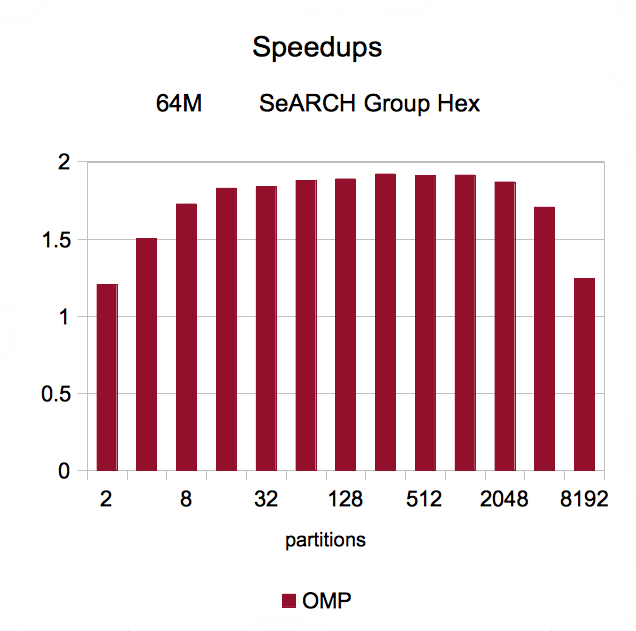
\includegraphics[width=\columnwidth]{images/hex-speedups-omp.png}
	\end{center}
	\caption{Speedups obtained for the shared memory version in the SeARCH Group Hex. The horizontal axis is in $\log_{2}$ scale and the refers to the number of partitions used. The vertical axis is in linear scale and shows the speedup achieved for each number of partitions.}
	\label{fig:omp}
\end{figure}

\Cref{fig:omp,fig:mpi} plot the achieved speedup values for each version. The reference value is the execution with only 1 partition.

As expected, the two graphs show an inverted bathtub curve. For the MPI implementation, the peak is achieved for 8 processes, one in each node. The test case with 16 processes reaches to values near the peak, but either the Intel\textregistered HyperThreading Technology or the two processes in each node competing for the same memory bank are keeping the system from achieving higher speedup values. From this case on, has the number of partitions increases, also do the number of processes, and consequently so does the communication overhead and the struggle for the resources in each node.

Regarding the OpenMP graph, the peak is achieved for 256 processes, but speedup values near this limit are achieved for a wide range of partitions. For numbers below the number of hardware threads the speedup values are lower due to underutilization of the computational resources. For numbers above 2048, the required structures that support the algorithm are likely bursting the cache, forcing to more RAM accesses which slow down the algorithm. This hypothesis should be verified with a deeper profiling but such study is out of the scope of this document.

\begin{figure}[t]
	\begin{center}
		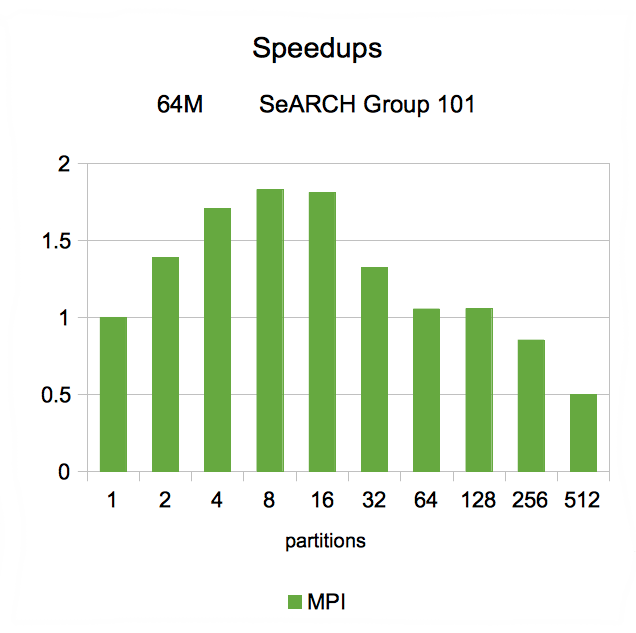
\includegraphics[width=\columnwidth]{images/101-speedups-mpi.png}
	\end{center}
	\caption{Speedups obtained for the distributed memory version in the SeARCH Group 101. The horizontal axis is in $\log_{2}$ scale and the refers to the number of partitions used. The vertical axis is in linear scale and shows the speedup achieved for each number of partitions.}
	\label{fig:mpi}
\end{figure}
		


\section{Conclusion}
In this document, the PSRS algorithm was described. It allows parallelism by selecting samples and pivots at regular intervals, which are then used to divide the already divided domain, in order to reduce data movement to the bare minimum.

Two implementations of this algorithm were presented. The first in distributed memory with OpenMPI and the second in shared memory with OpenMP. The two versions little differ, aside from the intrinsic need for one of them to perform external communications between processes.

Both versions were tested and measured for comparison. The peak for the shared memory version went way further than the number of threads available in the hardware, until it reached quantities which defy the limits of cache memory. As for the distributed memory version, the peak was measured to be the number of cores available. Whether this happened because of memory struggles for greater numbers of partitions, or because hardware features like the Intel\textregistered HyperThreading, such details are out of the scope of this document and therefore were not explored.

The obvious conclusion arises that this algorithm does not scale as well as expected. Yet, due to non published results regarding a similar experience, which reported considerably higher speedups, the question arises if the problem is not in the implementation.

As such, future work on this matter should start by checking bottlenecks in both versions. The roofline model would be a good starting point, from where it would be possible to see if the bound is computation or memory related. Other improvements can focus on studying and improving the implementation's locality and/or reducing communication (MPI).




\bibliographystyle{cell}
\bibliography{references}

\end{document}
